\chapter{Экономическое обоснование эффективности проекта}
\label{cha:wirtsch}

В данном разделе описаны экономические аспекты проекта по созданию ПО <<primiview>> для обработки геометрической информации 2D-объектов специального типа.

Целью экономического обоснования проекта является представление разработанного ПП в качестве проекта для реализации на предприятии, что позволит провести планирование и корректировку последовательности работ (при необходимости).

\section{Разработка проекта}

\textbf{Цель проекта} --- создание модуля конвертации форматов, как отдельного ПП, для внедрения в ПО для автоматизации технологического проектирования обработки деталей типа <<Втулка>> на станках с ЧПУ к 05.06.2023.

\textit{Обоснование цели}. Клиент --- это производитель станков с ЧПУ. Для создания УП на продаваемые станках клиенты заказчика привлекают САПР, разработанные за рубежом, что негативно влияет на независимость от сторонних организаций, ограниченность в дополнении ПО функционалом, необходимым только на отдельном предприятии, а также, на сохранность информации, используемой при разработке УП. Компания работает над проектом разработки своей CAM-системы для предложения своим клиентам специализированного ПО вместе с оборудованием с целью решить вышеуказанные проблемы. 

Численные критерии сравнения состояний системы клиента:
\begin{itemize}
	\item сложность проектирования,
	\item сроки (время) проектирования,
	\item себестоимость проектирования,
	\item качество результатов проектирования.
\end{itemize}

\textit{Пояснения к критериям}. Под сложностью проектирования понимается минимально-необходимая квалификация проектировщика для выполнения задач технологического проектирования.

Трудоёмкость проектирования, в данном случае, выражается в среднем времени создания (написания) одной УП.

Себестоимость проектирования оценивается не в расчёте на одну УП, а в рамках одного рабочего года. В себестоимость проектирования входят такие элементы, как зарплата сотрудника, производящего проектирование, а также, цена годовой лицензии/контракта обслуживания CAM-системы для данного количества оборудования на предприятии.

В качестве численного критерия для оценки качества результатов проектирования принято среднее количество типов ошибок, корректировки по которым оператор станка с ЧПУ вносит после того, как автоматизированное проектирование выполнено.

\textbf{Текущее состояние системы клиента}: основное ПО по автоматизации технологического проектирования введено в эксплуатацию, базовые потребности системы по конвертации DXF-файлов работают.

По численным критериям:
\begin{itemize}
	\item сложность проектирования: инженер-технолог II категории по квалификационному справочнику \cite{qualification},
	\item сроки (время) проектирования: 3 часа,
	\item себестоимость проектирования: 1420000 руб. (см. раздел \ref{par:ecocalc}),
	\item качество результатов проектирования: 10 ошибок.
\end{itemize}

Клиенты заказчика обращались с просьбами и пожеланиями, поставить им продукт, повышающий их эффективность по вышеуказанным критериям.

Клиенты заказчика испытывают трудности в удержании и поиске инженеров-технологов с высокой квалификацией (II категории), поэтому при возможности приобрести ПО, снижающее требования к квалификации инженеров-технологов, изъявили намерение купить такой ПП.

Несмотря на высокую квалификацию инженеров-технологов, занимающихся созданием УП, время проектирования сильно ограничивает мощностные способности клиентов заказчика. Заказчик ПО преследует интересы своих клиентов в сокращении времени проектирования ценой платы за специализированное ПО.

Клиенты заказчика стремятся повысить качество производимой продукции, поэтому нуждаются в дополнительных вложениях в соответствующие мероприятия. В качестве решения заказчик предложил снизить стоимость проектирования путём использования отечественного более дешёвого специального ПО.

Ещё одна причина заинтересованности клиентов заказчика в CAM-системе --- качество результатов проектирования. Оно напрямую влияет как на качество самой производимой продукции, так и на количество бракованных изделий. Снизить частоту и характер ошибок призвана разработанная САПР.

\textbf{Целевое состояние системы клиента}: усовершенствованная, более гибкая и универсальная версия этого ПО.

По численным критериям:
\begin{itemize}
	\item сложность проектирования: инженер-технолог (без категории) по квалификационному справочнику \cite{qualification},
	\item сроки (время) проектирования: максимум 1,5 часа,
	\item себестоимость проектирования: максимум 1 млн.руб.,
	\item качество результатов проектирования: максимум 5 типов ошибок.
\end{itemize}

\textbf{Результатом} проекта является факт конвертации файлов из формата DXF в форматы TXT(тип DXF), TXT(x,y,r), SVG, JSON, созданные в разработанном ПП. Файлы последних форматов содержат в себе геометрическое описание объектов по правилам, описанным в предыдущих разделах ВКР, из входного DXF, удобное для дальнейшей работы в CAM-системе "ТокКТЭ" и других САПР.

Команда проекта сформирована из 3 человек, среди которых:
\begin{enumerate}
	\item 1 владелец,
	\item 2 программиста, среди которых:
	\begin{enumerate}
		\item[б.1)] 1 разработчик,
		\item[б.2)] 1 тестировщик.
	\end{enumerate}
\end{enumerate}

Владелец проекта организует работу остальной команды, проводит планирование проекта, оценку его экономической эффективности, контроль за выполнением подчинёнными задач проекта.

Программисты занимаются непосредственно созданием продукта проекта, то есть написанием ПО. Разработчики отвечают за написание программного кода по техническому заданию проекта. Тестировщики выполняют проверку работоспособности ПП, ищут и сообщают отделу разработчиков о найденных и необходимых к устранению ошибок и недочётов программы.

\section{Дерево задач проекта}

Целью данного этапа является построение иерархического дерева, включающего в себя последовательное разбиение общей цели проекта на подцели и задачи.

\subsection{Первый уровень иерархии.}

Главной целью проекта, как уже было сказано, является разработка программного обеспечения <<primiview>> по конвертации файлов в формате DXF в форматы TXT, SVG, JSON. Данная цель в проекте единственная и находится на высшем уровне иерархии.

\subsection{Второй уровень иерархии.}

В целях определения и формализации цели, структуры и методов проекта, чтобы исключить неоднозначное их понимание и толкование исполнителями, первый этап, стоящий в иерархии на втором уровне, --- это \textit{формирование технического задания (ТЗ)}.

При параллельном методе разработке, когда этапы проекта могут начинаться тогда, пока предыдущие ещё не закончились, следующим шагом данного уровня будет \textit{разработка алгоритмов} программного обеспечения. Данный этап необходим, так как именно на нём ещё можно решить несостыковки в логической части программы, исправление которых на следующих этапах редко бывает возможным.

Параллельно с разработкой алгоритмов начинается этап непосредственно \textit{разработки ПО}. Эти этапе происходят одновременно, так как они тесно взаимосвязаны, и, например, не зная на каком ЯП будет разрабатываться ПО, трудно будет рационально подобрать алгоритмы, отвечающие возможностям ЯП.

Завершающим этапом второго уровня является \textit{сдача проекта} заказчику. Эта стадия может быть выполнена только при полном выполнении предыдущих стадий, если иное не было предварительно оговорено с заказчиком.

\subsection{Третий уровень иерархии.}

Этап формирования ТЗ подразделяется на следующие задачи:

\begin{enumerate}
	\item Определение назначения ПО. Здесь формализуются цели и функции ПП. Впоследующем, они вносятся в ТЗ. Это смысл выполнения проекта, то, к чему стремится вся его команда, что хочет получить в итоге заказчик;
	\item Исследование степени разработанности. На стадии предпроектного исследования выполняется проверка, существуют ли аналоги данного продукта в открытом доступе рынка. Если есть, то чем заказчика не устраивает их использование;
	\item Требования к продукту. Определяются численные критерии, которым должен соответствовать результат проекта на этапе его сдачи;
	\item Определение сроков. Всем участникам проекта необходимо знать, к какому сроку они должны выполнить определённый ранее объём работ. Сотрудникам, при согласовании ТЗ, необходимо оценить эти сроки, и в случае невозможности из соблюдения, просить корректировки и согласования с заказчиком более позднего выполнения задач;
	\item Написание ТЗ. Завершающая стадия этапа формирования ТЗ --- здесь собирается вся информация с предыдущих стадий и документируется согласно стандартам организации. ТЗ должно быть согласовано со всему участниками проекта.
\end{enumerate}

Этап разработки алгоритмов подразделяется на следующие стадии:
\begin{enumerate}
	\item Определение принципа работы ПО. Составляется принципиальная схема работы ПО, связь модулей, определяется предназначение каждого из модулей;
	\item Разработка алгоритмов для модулей ПП. Происходит решение поставленных задач на уровне логики и математики, строится набор взаимосвязей алгоритмов. По возможности, рассматривается применение уже существующих универсальных (реже, специальный) алгоритмов.
\end{enumerate}

Этап разработки ПО содержит такие стадии:
\begin{enumerate}
	\item Выбор ЯП. Данная стадия подразумевает проведение сравнительного анализа существующих инструментов различных ЯП применительно к разрабатываемому ПП;
	\item Определение структуры ПО. Эта стадия необходима для понимания разработчика функционала каждого из модулей программы. От этого зависит, на какие части (из каких файлов) будет состоять ПО;
	\item Написание и отладка программного кода. Главная часть создания продукта. На этой стадии разработчики непосредственно пишут программный код и отлаживают его работу.
	\item Тестирование ПО. Команда тестировщиков, также, пишет тестовый код, который проверяет разрабатываемое ПО на корректность работы его функционала.
\end{enumerate}

Завершающий этап на втором уровне иерархии --- сдача ПО, содержит следующие стадии:
\begin{enumerate}
	\item Презентация. Команда проекта презентует результаты своей работы заказчику, демонстрирует работу программы. Отчитывается по выполнению всех этапов, указанных в ТЗ;
	\item Внесение правок. По итогам презентации команда проекта заслушивает обратную связь от заказчика и на этой основе вносит в проект правки;
	\item Передача ПО заказчику. Организатор проекта передаёт заказчику исходный код ПО, документацию и инструкции, требования, прочие исходные файлы, информацию, обеспечивающую доступ к ПП;
	\item Обучение Сотрудников. При сдаче нового ПП, команде разработчиков необходимо обучить персонал заказчика работе с новым ПО;
	\item Устранение недостатков. После обучения исполнитель проекта (организация) предоставляет заказчику 7 рабочих дней на проведение внутренних проверок ПО, по результатам которых заказчик предоставляет исполнителю список исправлений, которые команда проекта обязана скорректировать в разработанном ПО;
	\item Закрытие задания на проект. Расчёт. Конечным мероприятием сдачи ПО являет закрытие сторонами задания по договору и получение расчёта за выполненную работую.
\end{enumerate}

\subsection{Четвёртый уровень иерархии.}

Описание данного уровня иерархии приведено кратко для примера. В самом деле, каждая из стадий третьего уровня подразделяется на задачи четвёртого уровня.

Стадия исследования степени разработанности проблемы в этапе формирования ТЗ подразделяется на следующие задачи:
\begin{enumerate}
	\item Исследование отечественного рынка аналогичных ПП. Задача состоит в поиске решений по аналогичным проектам в открытом доступе в рамках отчественного рынка;
	\item Исследование зарубежного рынка аналогичных ПП. Данная задача отличается от предыдущей сложностью поиска аналогов (на зарубежном рынке(пространстве)), так как для проведения данного анализа необходим высокий уровень владения иностранным (английским) языком, а также, требуется знание достоверных ресурсов (источников) информации.
\end{enumerate}

Описанные элементы иерархии сведены в иерархическое дерево (см. рисунок \ref{fig:projektaufgaben}). Уровни иерархической структуры оформлены таким образом, что, чем конкретнее описаны элементы структуры, тем насыщеннее цвет заливки.

	
\begin{figure}[H]
	\centering
	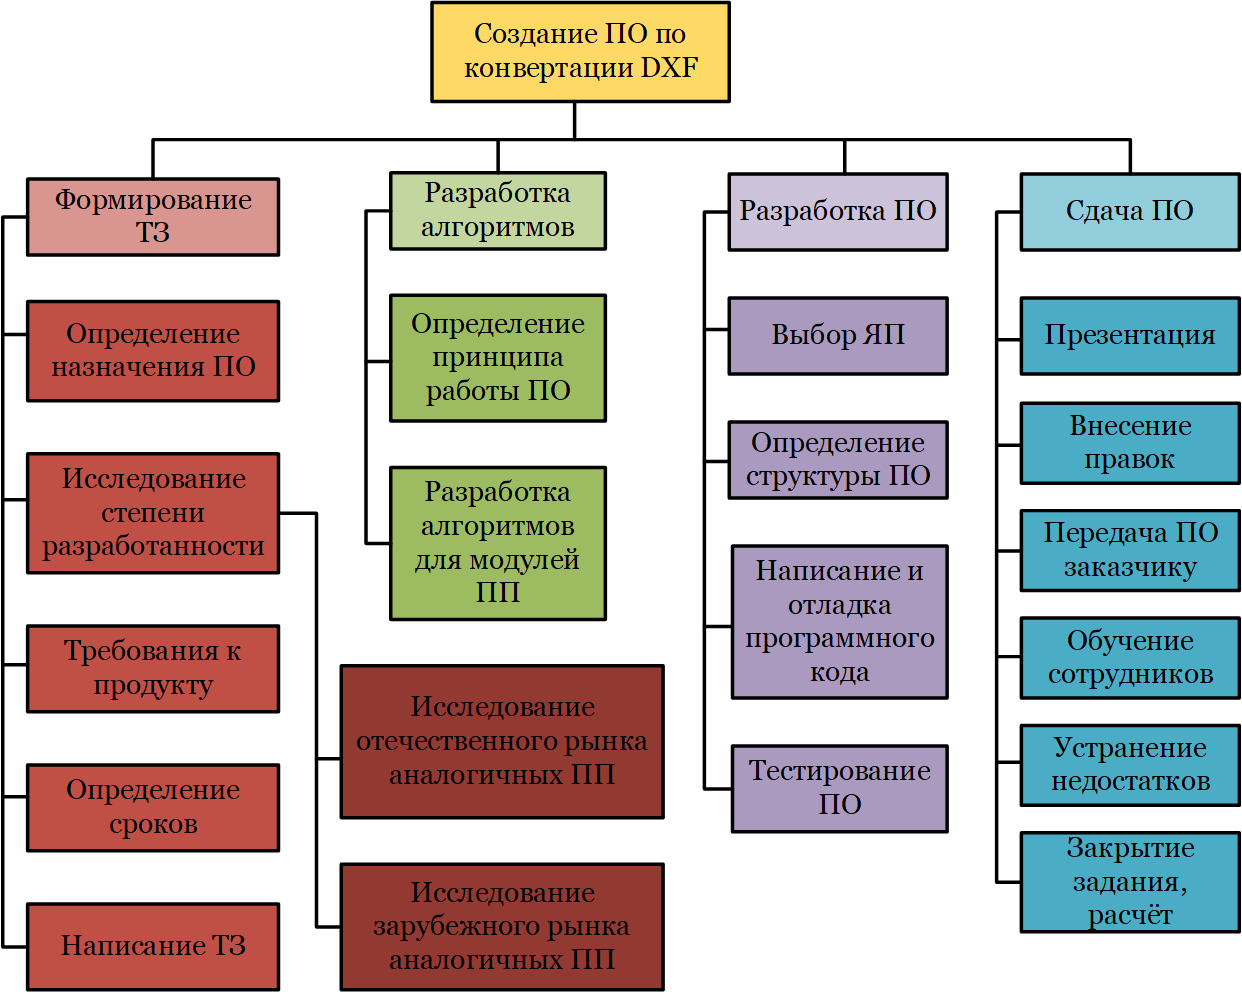
\includegraphics[width=1.0\textwidth]{figures/projektaufgaben.png}
	\captionof{figure}{Дерево задач проекта}
	\label{fig:projektaufgaben}
\end{figure}

\section{Построение диаграмм проекта}

В целях визуализации информации в области планирования проекта, а также для удобства, наглядности и гибкости контроля за выполнением задач проекта используются методы построения диаграмм и графов проекта.

\subsection{Диаграмма Ганта}

На данном этапе строится диаграмма Ганта (англ. Gantt Chart, также, ленточная диаграмма, график Ганта) --- это тип столбчатых диаграмм, использующийся для иллюстрации плана, графика работ проекта. Изобрёл такой тип диаграмм американский <<прародитель>> менеджмента Генри Лоренс Гант \cite{gantt}. Также, является методом планирования проекта. Эта диаграмма представляет собой отрезки (графические плашки), размещающиеся на горизонтальной шкале времени. Каждый отрезок соответствует отдельно задаче (подзадаче). Начало, конец и длина отрезка на шкале времени соответствуют началу, концу и длительности задачи. Диаграмма может использоваться для представления текущего состояния выполнения работ: часть прямоугольника, отвечающего задаче, заштриховывается, отмечая процент выполнения задачи; показывается вертикальная линия, отвечающая моменту «сегодня».

Рядом с самой диаграммой располагается таблица со списком работ, строки которой соответствуют отдельным задачам, отображённым на диаграмме, в то время как столбцы содержат дополнительную информацию о задаче.


%\begin{sidewaysfigure}[H]
%	\centering
%	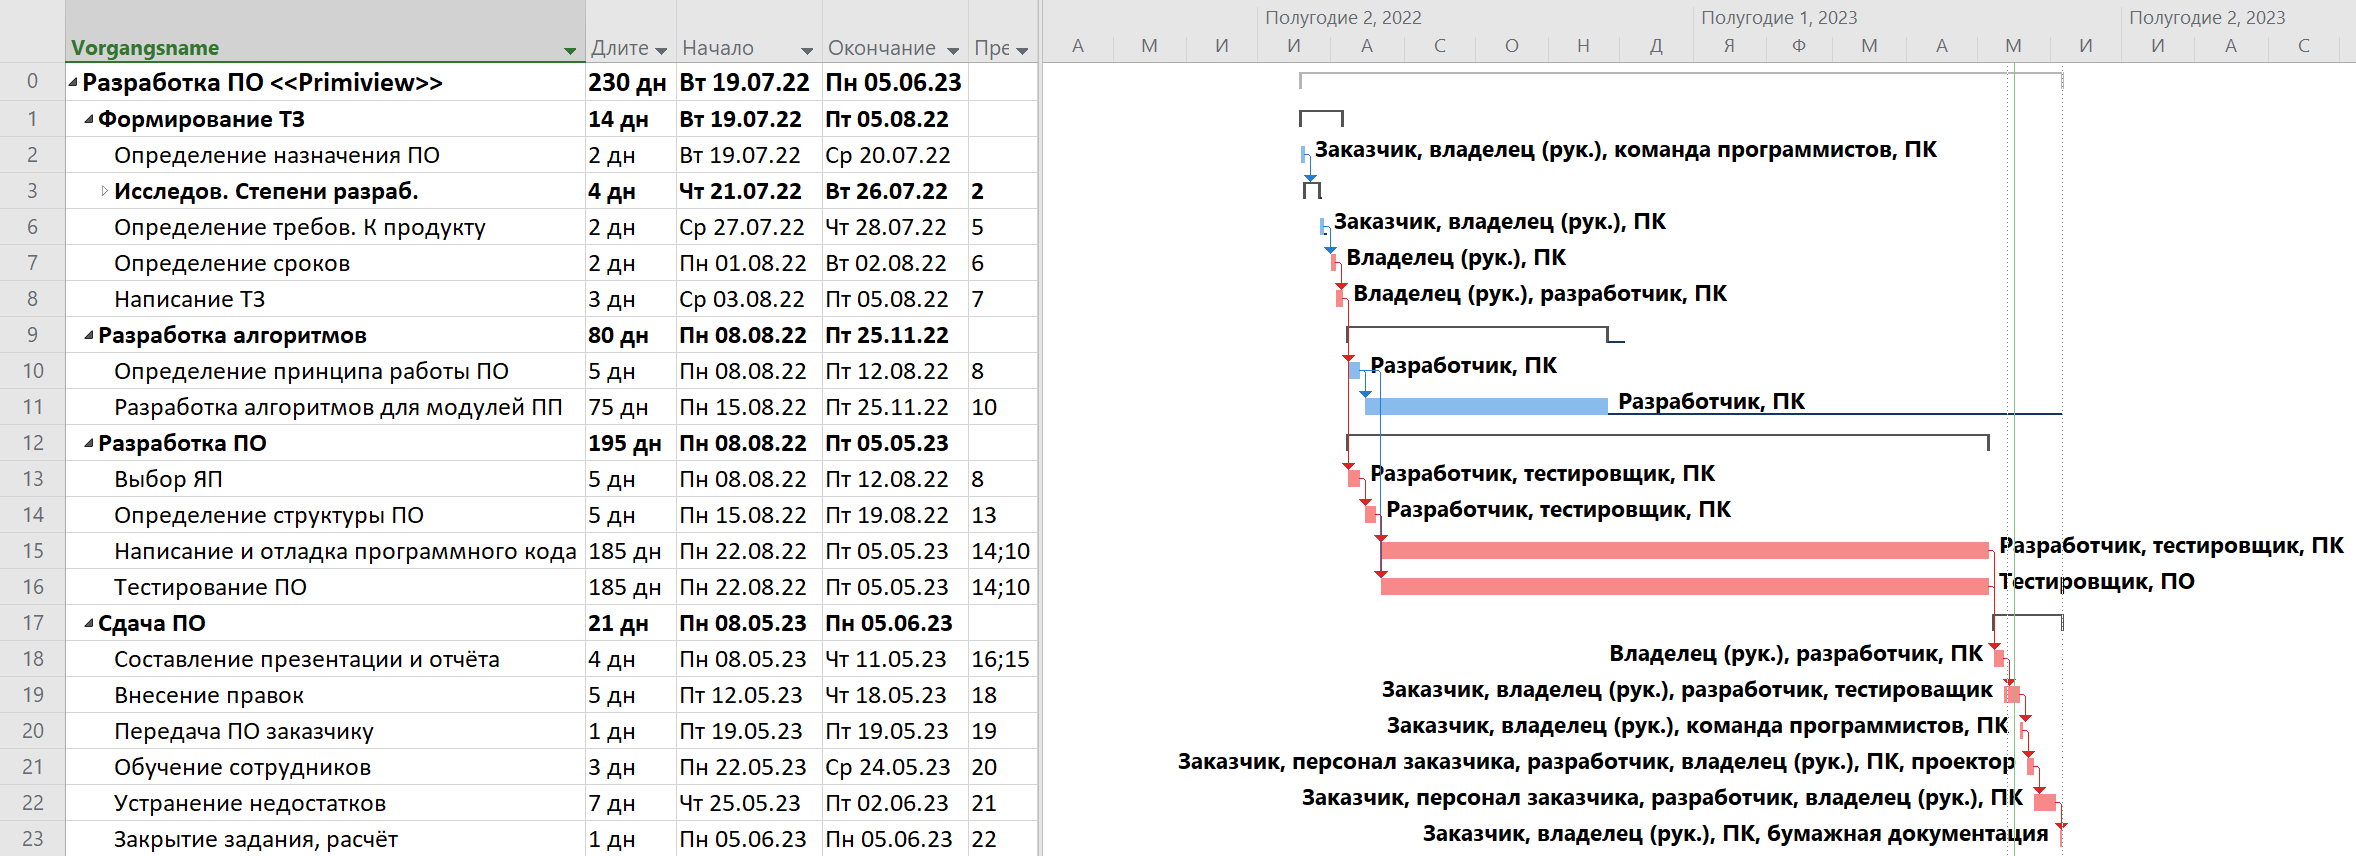
\includegraphics[width=\textwidth, height=0.5\textheight]{figures/gantt.png}
%	\captionof{figure}{Диаграмма Ганта для проекта}
%	\label{fig:gantt}
%\end{sidewaysfigure}


%\begin{landscape}
%\begin{sideways}
%\KOMAoptions{paper=landscape, pagesize}
%\recalctypearea
%\begin{landscape}
\begin{figure}[H]
	\centering
	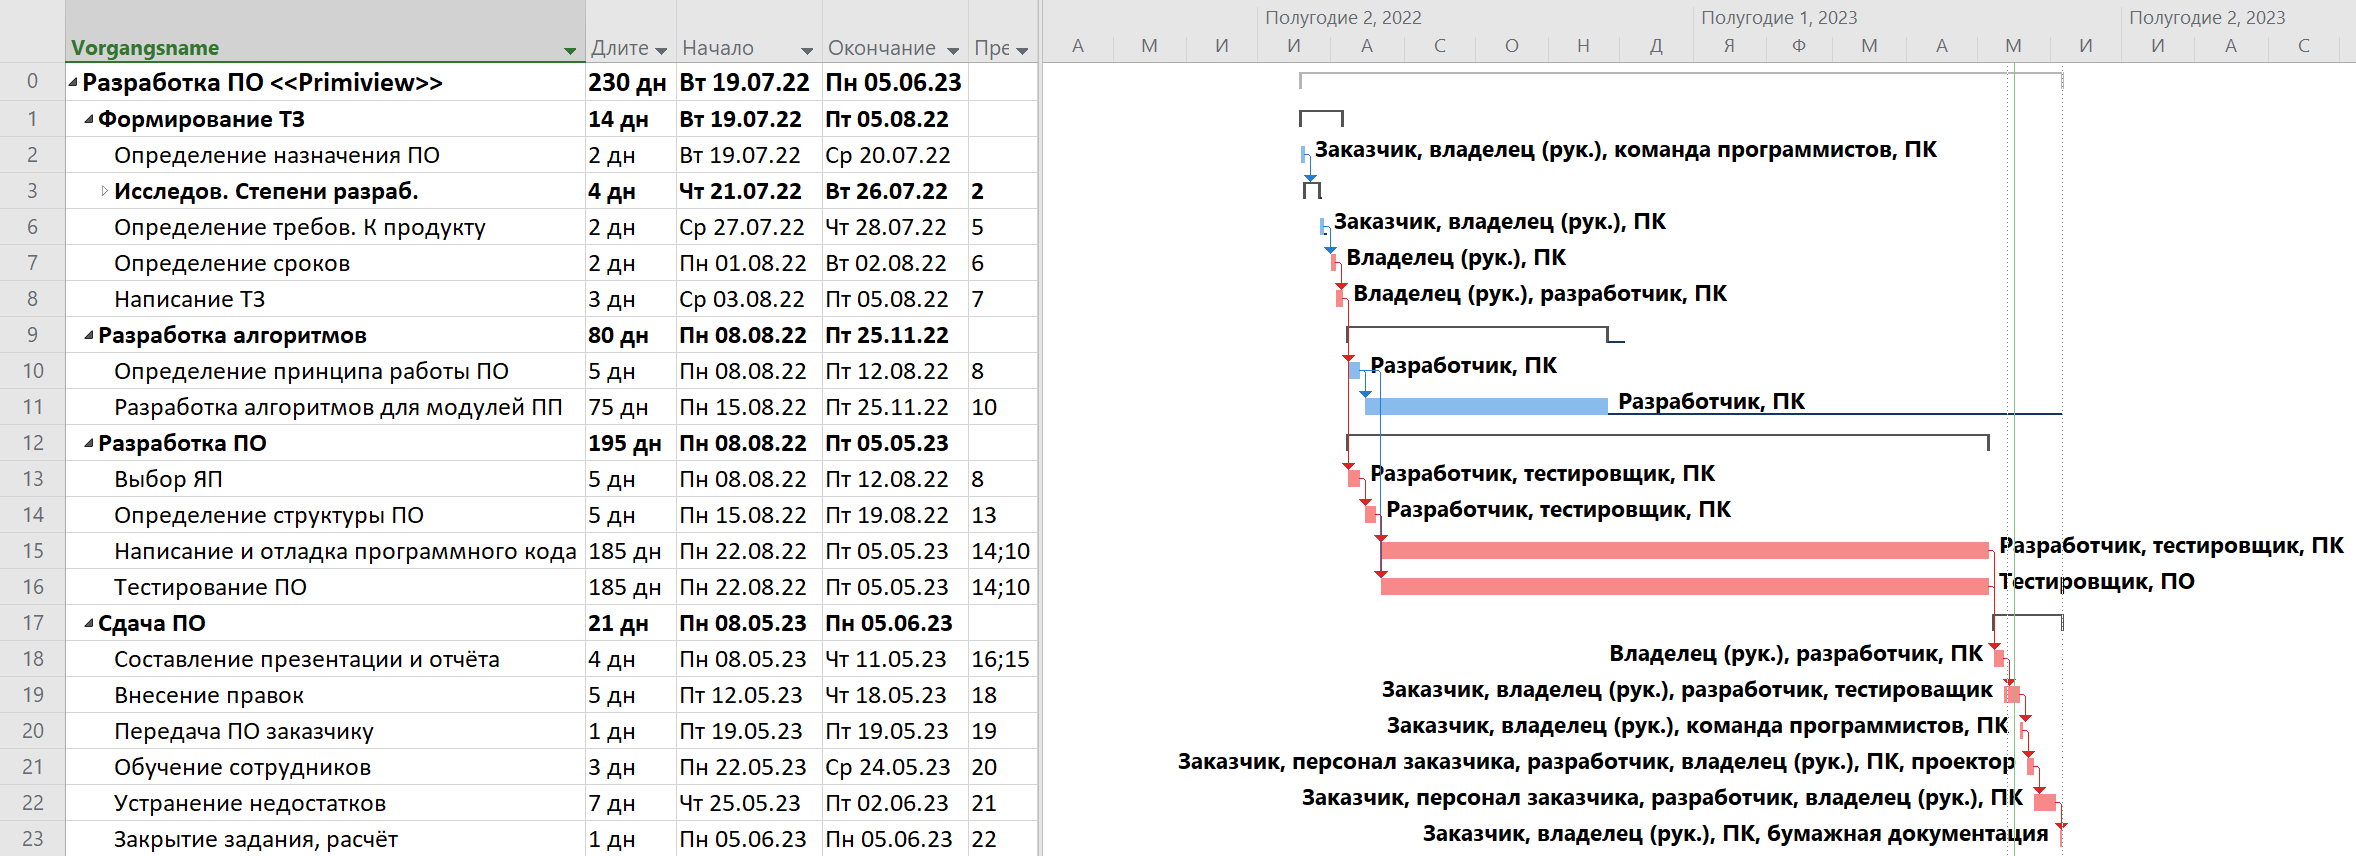
\includegraphics[width=1.4\textwidth, angle=90]{figures/gantt.png}
	\captionof{figure}{Диаграмма Ганта для проекта}
	\label{fig:gantt}
\end{figure}
%\end{landscape}
%\KOMAoptions{paper=portrait, pagesize}
%\recalctypearea
%\end{sideways}
%\end{landscape}

\subsection{Сетевой график}

С целью точного определения плановых сроков завершения проекта и выявления потенциальных вариантов их сокращения, а также для выявления и планирования критического пути проекта строится сетевой график.

Сетевой график представляет собой ориентированный граф, изображающий все необходимые для достижения цели проекта операции в технологической взаимосвязи. Другими словами, это изображение комплекса работ с учётом их длительности, взаимосвязи и перечнем неделимых операций в порядке их выполнения.

Основной элемент сетевого графика --- события, характеризующие завершение или начало работы. Оно обычно обозначается окружностью внутри которой располагается номер события (для сверки со справочной таблицей, прилагающейся к сетевому графику).

Стрелками на сетевом графике изображаются работы --- реальные процессы или действия, требующие затрат труда, материалов и времени, и приводящие к событию, на которое обращена стрелка. Работы на сетевом графике обычно означают одно из следующего:
\begin{itemize}
	\item Действительная работа --- производственный или творческий процесс, требующий усилий, затрат труда, времени и материальных ресурсов;
	\item Ожидание --- процесс, требующий только затрат времени без привлечения каких-либо ресурсов;
	\item Зависимость (фиктивная работы) --- процесс, не требующий затрат труда, времени и ресурсов.
\end{itemize}

Продолжительность работы для проектов на глобальном уровне обычно измеряется, как минимум, днями. Однако на разной масштабности может также и быть оценена в часах, неделях, месяцах, годах. Работы могут иметь количественные показатели, характеризующие трудоёмкость, стоимость, материальные ресурсы.

Временные показатели изображаются над стрелками, обозначение работ --- под стрелками.

К сетевым графикам предъявляется требование, чтобы события были определены полно и чётко, их формулировка должна включать результат предшествующих ему работ. Если то или иное событие наступило, то это значит, что сразу могут быть начаты следующие работы.

Путь на сетевом графике --- это непрерывная последовательность работ от исходного до завершающего события.

Критическим путём называется путь сетевого графика с наибольшей суммарной продолжительностью работ.

При построении сетевых графиков необходимо придерживаться следующих правил:
\begin{enumerate}
	\item Последовательное изображение работ от начала к окончанию,
	\item Изображение стрелок от предшествующего события к последующему,
	\item Отсутствие пересечения стрелок,
	\item Обозначение работ: между двумя событиями только одна стрелка,
	\item Запрет на замкнутые контуры, тупики, хвостовые работы,
	\item Изображение дифференциально-зависимых работ с помощью пунктирных стрелок,
	\item Изображение поставки-результата внешней работы, используемого в данной работе,
	\item Кодирование событий.
\end{enumerate}

Согласно описанным принципам построения сетевых графиков был разработан сетевой график для проекта по разработке ПО <<primiview>> для конвертирования файлов. На рисунке \ref{fig:netzkompakt} изображена сама сеть. Для расшифровки событий и работ см. таблицы \ref{tab:netzarbeiten} и \ref{tab:netzersch}.

\begin{figure}[H]
	\centering
	\includegraphics[width=\textwidth, angle=0]{figures/netzkompakt.png}
	\captionof{figure}{Сетевой график проекта}
	\label{fig:netzkompakt}
\end{figure}

\begin{longtable}{|m{0.06\textwidth}|p{0.57\textwidth}|m{0.08\textwidth}|m{0.10\textwidth}|}
	\caption{Работы в сетевом графике проекта}
	\label{tab:netzarbeiten}
	\centering
	\tabularnewline
	\hline
	\multicolumn{1}{|m{0.10\textwidth}|}{Обозн.}&\multicolumn{1}{c|}{Наименование этапа}&\multicolumn{1}{m{0.12\textwidth}|}{Продолж.\newline (раб. дней)}&\multicolumn{1}{m{0.10\textwidth}|}{Предш. этап}\\
	\hline \endfirsthead
	\subcaption{Продолжение таблицы~\ref{tab:netzarbeiten}}\\
	\hline \endhead
	\subcaption{Продолжение на след. стр.}
	\endfoot
	%\hline
	\endlastfoot
	A&Принятие командой проекта решений по назначению ПО, исследование аналогов, определение требований и сроков&14&-\\ \hline
	B&Определение файловых потоков&2&A\\ \hline
	C&Определение взаимосвязи файлов ПО&3&B\\ \hline
	D&Сравнение концепций хранения данных внутри ПО, схематизация и моделирование вариантов реализации алгоритма, проверка алгоритма на ошибки&10&C\\ \hline
	E&Вывод зависимостей между доступными параметрами дуг и необходимой геометрией дуг, разработка алгоритма&10&C\\ \hline
	F&Разработка алгоритма по перебору и внутрепрограммному сохранению координат изображения&10&C\\ \hline
	G&Разработка алгоритма на основе созданной структуры хранения примитивов&10&D\\ \hline
	H&Разработка алгоритма с использованием созданных алгоритмов вычленения необходимой информации из DXF-файлов&10&E\\ \hline
	I&Применение встроенных в ЯП методов сортировки, применение предыдущего алгоритма&2&F\\ \hline
	J&Выполнение операций над краевыми значениями массивов координат&1&F\\ \hline
	K&Разработка алгоритма конвертации с использованием радиуса сегмента полилиний&5&G,H\\ \hline
	L&Разработка алгоритма конвертации с использованием альтернативного метода описания дуг&10&J\\ \hline
	M&Разработка алгоритма с использованием встроенных в ЯП алгоритмов сортировки&2&I\\ \hline
	N&Разработка алгоритма с использованием извлечённых из DXF Геометрических данным для визуализации изображения&5&H,K\\ \hline
	O&Разработка алгоритма конвертации DXF В JSON с объединением примитивов в контуры&10&L,M,N\\ \hline
	P&Сравнительный анализ ЯП в применении к поставленным требованиям к ПО&5&O\\ \hline
	Q&Написание кода программы и его отладка&138&P\\ \hline
	R&Тестирование функционала разработанного ПО&138&Q\\ \hline
	S&Подготовка документа-отчёта, а также составление презентации с подготовкой команды проекта к демонстрации разработанного ПП&4&R\\ \hline
	T&Подготовка презентации и отчёта с незавершёнными тестами ПО&2&Q\\ \hline
	U&Заслушивание обратной связи заказчика после презентации. Составление списка замечаний к исправлению&6&S,T\\ \hline
	V&Проведение обучения сотрудников заказчика к пользованию ПП. Передача ПО заказчику. Предоставление времени на внутреннюю проверку нового ПО&10&U\\ \hline
	W&Приём списка замечаний сотрудников заказчика после периода внутренней апробации ПП&7&V\\ \hline
	X&Обновление переданного ПО заказчику. Завершающая встреча заказчика и владельца проекта для подписания оформленных к завершению проекта документов&1&W\\ \hline
\end{longtable}

\begin{longtable}{|m{0.06\textwidth}|p{0.70\textwidth}|m{0.10\textwidth}|}
	\caption{События в сетевом графике проекта}
	\label{tab:netzersch}
	\centering
	\tabularnewline
	\hline
	\multicolumn{1}{|m{0.10\textwidth}|}{Обозн.}&\multicolumn{1}{c|}{Наименование события}&\multicolumn{1}{m{0.12\textwidth}|}{Предш. событие}\\
	\hline \endfirsthead
	\subcaption{Продолжение таблицы~\ref{tab:netzersch}}\\
	\hline \endhead
	\subcaption{Продолжение на след. стр.}
	\endfoot
	%\hline
	\endlastfoot
	1&Начало проекта&-\\ \hline
	2&Техническое задание&1\\ \hline
	3&Схема работы ПО&2\\ \hline
	4&Структура ПО&3\\ \hline
	5&Алгоритм внутрепрограммного сохранения примитивов&4\\ \hline
	6&Алгоритм вычисления радиуса сегмента полилинии&4\\ \hline
	7&Алгоритм вычленения координат из объектов DXF&4\\ \hline
	8&Алгоритм конвертации DXF$\rightarrow$TXT(DXF-type)&5\\ \hline
	9&Алгоритм поиска наименьших координат изображения&7\\ \hline
	10&Алгоритм поиска ширины и высоты рамки объектов DXF&7\\ \hline
	11&Алгоритм конвертации DXF$\rightarrow$TXT(x,y,r)&6,8\\ \hline
	12&Алгоритм конвертации DXF$\rightarrow$SVG&9,10,11\\ \hline
	13&Алгоритм конвертации DXF$\rightarrow$JSON&12\\ \hline
	14&Утверждённый руководителем проекта ЯП&13\\ \hline
	15&Файлы проекта с исходным кодом&14\\ \hline
	16&Отчёт о прохождении тестов&15\\ \hline
	17&Презентация и отчёт проекта в эл.виде&16\\ \hline
	18&Список правок&17\\ \hline
	19&Результаты тестирования сотрудников&18\\ \hline
	20&Список устранённых недостатков&19\\ \hline
	21&Подписанное о закрытии задание проекта. Счёт на оплату. Чек об оплате&20\\ \hline
\end{longtable}


\section{Расчёт стоимости проекта}

Ресурс — средства, позволяющие с помощью определённых преобразований получить желаемый результат. 

После того как определен состав задач, необходимо определить, кто эти задачи будет исполнять и какое оборудование будет использоваться. Для этого нужно ввести в план проекта список ресурсов и информацию о них, а затем распределить эти ресурсы между задачами. 

С задачами, для которых назначены сроки, должны быть ассоциировано оборудование, средства и люди. Это подразумевает распределение обязанностей. Эта деятельность определяется и ограничивается доступностью ресурсов, их оптимальным использованием в заданном контексте и вопросами, связанными с персоналом.  

Для того чтобы определить стоимость всего проекта, необходимо обозначить виды ресурсов, стоимость этих ресурсов, время использования и необходимый объем.

\begin{figure}[H]
	\centering
	\includegraphics[width=1.0\textwidth]{figures/restable.png}
	\captionof{figure}{Распределение использования ресурсов}
	\label{fig:restable}
\end{figure} 

% save a table just in case. Import on https://www.latex-tables.com/
%\begin{longtblr}[
%	label = none,
%	entry = none,
%	]{
%		row{1} = {c},
%		row{2} = {c},
%		cell{1}{1} = {r=2}{},
%		cell{1}{2} = {r=2}{},
%		cell{1}{3} = {r=2}{},
%		cell{1}{4} = {c=12}{},
%		cell{3}{1} = {r=11}{c},
%		cell{3}{3} = {c},
%		cell{3}{4} = {c},
%		cell{3}{5} = {c},
%		cell{3}{6} = {c},
%		cell{3}{7} = {c},
%		cell{3}{8} = {c},
%		cell{3}{9} = {c},
%		cell{3}{10} = {c},
%		cell{3}{11} = {c},
%		cell{3}{12} = {c},
%		cell{3}{13} = {c},
%		cell{3}{14} = {c},
%		cell{3}{15} = {c},
%		cell{4}{3} = {c},
%		cell{4}{4} = {c},
%		cell{4}{5} = {c},
%		cell{4}{6} = {c},
%		cell{4}{7} = {c},
%		cell{4}{8} = {c},
%		cell{4}{9} = {c},
%		cell{4}{10} = {c},
%		cell{4}{11} = {c},
%		cell{4}{12} = {c},
%		cell{4}{13} = {c},
%		cell{4}{14} = {c},
%		cell{4}{15} = {c},
%		cell{5}{3} = {c},
%		cell{5}{4} = {c},
%		cell{5}{5} = {c},
%		cell{5}{6} = {c},
%		cell{5}{7} = {c},
%		cell{5}{8} = {c},
%		cell{5}{9} = {c},
%		cell{5}{10} = {c},
%		cell{5}{11} = {c},
%		cell{5}{12} = {c},
%		cell{5}{13} = {c},
%		cell{5}{14} = {c},
%		cell{5}{15} = {c},
%		cell{6}{3} = {c},
%		cell{6}{4} = {c},
%		cell{6}{5} = {c},
%		cell{6}{6} = {c},
%		cell{6}{7} = {c},
%		cell{6}{8} = {c},
%		cell{6}{9} = {c},
%		cell{6}{10} = {c},
%		cell{6}{11} = {c},
%		cell{6}{12} = {c},
%		cell{6}{13} = {c},
%		cell{6}{14} = {c},
%		cell{6}{15} = {c},
%		cell{7}{3} = {c},
%		cell{7}{4} = {c},
%		cell{7}{5} = {c},
%		cell{7}{6} = {c},
%		cell{7}{7} = {c},
%		cell{7}{8} = {c},
%		cell{7}{9} = {c},
%		cell{7}{10} = {c},
%		cell{7}{11} = {c},
%		cell{7}{12} = {c},
%		cell{7}{13} = {c},
%		cell{7}{14} = {c},
%		cell{7}{15} = {c},
%		cell{8}{3} = {c},
%		cell{8}{4} = {c},
%		cell{8}{5} = {c},
%		cell{8}{6} = {c},
%		cell{8}{7} = {c},
%		cell{8}{8} = {c},
%		cell{8}{9} = {c},
%		cell{8}{10} = {c},
%		cell{8}{11} = {c},
%		cell{8}{12} = {c},
%		cell{8}{13} = {c},
%		cell{8}{14} = {c},
%		cell{8}{15} = {c},
%		cell{9}{3} = {c},
%		cell{9}{4} = {c},
%		cell{9}{5} = {c},
%		cell{9}{6} = {c},
%		cell{9}{7} = {c},
%		cell{9}{8} = {c},
%		cell{9}{9} = {c},
%		cell{9}{10} = {c},
%		cell{9}{11} = {c},
%		cell{9}{12} = {c},
%		cell{9}{13} = {c},
%		cell{9}{14} = {c},
%		cell{9}{15} = {c},
%		cell{10}{3} = {c},
%		cell{10}{4} = {c},
%		cell{10}{5} = {c},
%		cell{10}{6} = {c},
%		cell{10}{7} = {c},
%		cell{10}{8} = {c},
%		cell{10}{9} = {c},
%		cell{10}{10} = {c},
%		cell{10}{11} = {c},
%		cell{10}{12} = {c},
%		cell{10}{13} = {c},
%		cell{10}{14} = {c},
%		cell{10}{15} = {c},
%		cell{11}{3} = {c},
%		cell{11}{4} = {c},
%		cell{11}{5} = {c},
%		cell{11}{6} = {c},
%		cell{11}{7} = {c},
%		cell{11}{8} = {c},
%		cell{11}{9} = {c},
%		cell{11}{10} = {c},
%		cell{11}{11} = {c},
%		cell{11}{12} = {c},
%		cell{11}{13} = {c},
%		cell{11}{14} = {c},
%		cell{11}{15} = {c},
%		cell{12}{3} = {c},
%		cell{12}{4} = {c},
%		cell{12}{5} = {c},
%		cell{12}{6} = {c},
%		cell{12}{7} = {c},
%		cell{12}{8} = {c},
%		cell{12}{9} = {c},
%		cell{12}{10} = {c},
%		cell{12}{11} = {c},
%		cell{12}{12} = {c},
%		cell{12}{13} = {c},
%		cell{12}{14} = {c},
%		cell{12}{15} = {c},
%		cell{13}{3} = {c},
%		cell{13}{4} = {c},
%		cell{13}{5} = {c},
%		cell{13}{6} = {c},
%		cell{13}{7} = {c},
%		cell{13}{8} = {c},
%		cell{13}{9} = {c},
%		cell{13}{10} = {c},
%		cell{13}{11} = {c},
%		cell{13}{12} = {c},
%		cell{13}{13} = {c},
%		cell{13}{14} = {c},
%		cell{13}{15} = {c},
%		cell{14}{1} = {r=13}{c},
%		cell{14}{3} = {c},
%		cell{14}{4} = {c},
%		cell{14}{5} = {c},
%		cell{14}{6} = {c},
%		cell{14}{7} = {c},
%		cell{14}{8} = {c},
%		cell{14}{9} = {c},
%		cell{14}{10} = {c},
%		cell{14}{11} = {c},
%		cell{14}{12} = {c},
%		cell{14}{13} = {c},
%		cell{14}{14} = {c},
%		cell{14}{15} = {c},
%		cell{15}{3} = {c},
%		cell{15}{4} = {c},
%		cell{15}{5} = {c},
%		cell{15}{6} = {c},
%		cell{15}{7} = {c},
%		cell{15}{8} = {c},
%		cell{15}{9} = {c},
%		cell{15}{10} = {c},
%		cell{15}{11} = {c},
%		cell{15}{12} = {c},
%		cell{15}{13} = {c},
%		cell{15}{14} = {c},
%		cell{15}{15} = {c},
%		cell{16}{3} = {c},
%		cell{16}{4} = {c},
%		cell{16}{5} = {c},
%		cell{16}{6} = {c},
%		cell{16}{7} = {c},
%		cell{16}{8} = {c},
%		cell{16}{9} = {c},
%		cell{16}{10} = {c},
%		cell{16}{11} = {c},
%		cell{16}{12} = {c},
%		cell{16}{13} = {c},
%		cell{16}{14} = {c},
%		cell{16}{15} = {c},
%		cell{17}{3} = {c},
%		cell{17}{4} = {c},
%		cell{17}{5} = {c},
%		cell{17}{6} = {c},
%		cell{17}{7} = {c},
%		cell{17}{8} = {c},
%		cell{17}{9} = {c},
%		cell{17}{10} = {c},
%		cell{17}{11} = {c},
%		cell{17}{12} = {c},
%		cell{17}{13} = {c},
%		cell{17}{14} = {c},
%		cell{17}{15} = {c},
%		cell{18}{3} = {c},
%		cell{18}{4} = {c},
%		cell{18}{5} = {c},
%		cell{18}{6} = {c},
%		cell{18}{7} = {c},
%		cell{18}{8} = {c},
%		cell{18}{9} = {c},
%		cell{18}{10} = {c},
%		cell{18}{11} = {c},
%		cell{18}{12} = {c},
%		cell{18}{13} = {c},
%		cell{18}{14} = {c},
%		cell{18}{15} = {c},
%		cell{19}{3} = {c},
%		cell{19}{4} = {c},
%		cell{19}{5} = {c},
%		cell{19}{6} = {c},
%		cell{19}{7} = {c},
%		cell{19}{8} = {c},
%		cell{19}{9} = {c},
%		cell{19}{10} = {c},
%		cell{19}{11} = {c},
%		cell{19}{12} = {c},
%		cell{19}{13} = {c},
%		cell{19}{14} = {c},
%		cell{19}{15} = {c},
%		cell{20}{3} = {c},
%		cell{20}{4} = {c},
%		cell{20}{5} = {c},
%		cell{20}{6} = {c},
%		cell{20}{7} = {c},
%		cell{20}{8} = {c},
%		cell{20}{9} = {c},
%		cell{20}{10} = {c},
%		cell{20}{11} = {c},
%		cell{20}{12} = {c},
%		cell{20}{13} = {c},
%		cell{20}{14} = {c},
%		cell{20}{15} = {c},
%		cell{21}{3} = {c},
%		cell{21}{4} = {c},
%		cell{21}{5} = {c},
%		cell{21}{6} = {c},
%		cell{21}{7} = {c},
%		cell{21}{8} = {c},
%		cell{21}{9} = {c},
%		cell{21}{10} = {c},
%		cell{21}{11} = {c},
%		cell{21}{12} = {c},
%		cell{21}{13} = {c},
%		cell{21}{14} = {c},
%		cell{21}{15} = {c},
%		cell{22}{3} = {c},
%		cell{22}{4} = {c},
%		cell{22}{5} = {c},
%		cell{22}{6} = {c},
%		cell{22}{7} = {c},
%		cell{22}{8} = {c},
%		cell{22}{9} = {c},
%		cell{22}{10} = {c},
%		cell{22}{11} = {c},
%		cell{22}{12} = {c},
%		cell{22}{13} = {c},
%		cell{22}{14} = {c},
%		cell{22}{15} = {c},
%		cell{23}{3} = {c},
%		cell{23}{4} = {c},
%		cell{23}{5} = {c},
%		cell{23}{6} = {c},
%		cell{23}{7} = {c},
%		cell{23}{8} = {c},
%		cell{23}{9} = {c},
%		cell{23}{10} = {c},
%		cell{23}{11} = {c},
%		cell{23}{12} = {c},
%		cell{23}{13} = {c},
%		cell{23}{14} = {c},
%		cell{23}{15} = {c},
%		cell{24}{3} = {c},
%		cell{24}{4} = {c},
%		cell{24}{5} = {c},
%		cell{24}{6} = {c},
%		cell{24}{7} = {c},
%		cell{24}{8} = {c},
%		cell{24}{9} = {c},
%		cell{24}{10} = {c},
%		cell{24}{11} = {c},
%		cell{24}{12} = {c},
%		cell{24}{13} = {c},
%		cell{24}{14} = {c},
%		cell{24}{15} = {c},
%		cell{25}{3} = {c},
%		cell{25}{4} = {c},
%		cell{25}{5} = {c},
%		cell{25}{6} = {c},
%		cell{25}{7} = {c},
%		cell{25}{8} = {c},
%		cell{25}{9} = {c},
%		cell{25}{10} = {c},
%		cell{25}{11} = {c},
%		cell{25}{12} = {c},
%		cell{25}{13} = {c},
%		cell{25}{14} = {c},
%		cell{25}{15} = {c},
%		cell{26}{3} = {c},
%		cell{26}{4} = {c},
%		cell{26}{5} = {c},
%		cell{26}{6} = {c},
%		cell{26}{7} = {c},
%		cell{26}{8} = {c},
%		cell{26}{9} = {c},
%		cell{26}{10} = {c},
%		cell{26}{11} = {c},
%		cell{26}{12} = {c},
%		cell{26}{13} = {c},
%		cell{26}{14} = {c},
%		cell{26}{15} = {c},
%		cell{27}{1} = {r=7}{c},
%		cell{27}{3} = {c},
%		cell{27}{4} = {c},
%		cell{27}{5} = {c},
%		cell{27}{6} = {c},
%		cell{27}{7} = {c},
%		cell{27}{8} = {c},
%		cell{27}{9} = {c},
%		cell{27}{10} = {c},
%		cell{27}{11} = {c},
%		cell{27}{12} = {c},
%		cell{27}{13} = {c},
%		cell{27}{14} = {c},
%		cell{27}{15} = {c},
%		cell{28}{3} = {c},
%		cell{28}{4} = {c},
%		cell{28}{5} = {c},
%		cell{28}{6} = {c},
%		cell{28}{7} = {c},
%		cell{28}{8} = {c},
%		cell{28}{9} = {c},
%		cell{28}{10} = {c},
%		cell{28}{11} = {c},
%		cell{28}{12} = {c},
%		cell{28}{13} = {c},
%		cell{28}{14} = {c},
%		cell{28}{15} = {c},
%		cell{29}{3} = {c},
%		cell{29}{4} = {c},
%		cell{29}{5} = {c},
%		cell{29}{6} = {c},
%		cell{29}{7} = {c},
%		cell{29}{8} = {c},
%		cell{29}{9} = {c},
%		cell{29}{10} = {c},
%		cell{29}{11} = {c},
%		cell{29}{12} = {c},
%		cell{29}{13} = {c},
%		cell{29}{14} = {c},
%		cell{29}{15} = {c},
%		cell{30}{3} = {c},
%		cell{30}{4} = {c},
%		cell{30}{5} = {c},
%		cell{30}{6} = {c},
%		cell{30}{7} = {c},
%		cell{30}{8} = {c},
%		cell{30}{9} = {c},
%		cell{30}{10} = {c},
%		cell{30}{11} = {c},
%		cell{30}{12} = {c},
%		cell{30}{13} = {c},
%		cell{30}{14} = {c},
%		cell{30}{15} = {c},
%		cell{31}{3} = {c},
%		cell{31}{4} = {c},
%		cell{31}{5} = {c},
%		cell{31}{6} = {c},
%		cell{31}{7} = {c},
%		cell{31}{8} = {c},
%		cell{31}{9} = {c},
%		cell{31}{10} = {c},
%		cell{31}{11} = {c},
%		cell{31}{12} = {c},
%		cell{31}{13} = {c},
%		cell{31}{14} = {c},
%		cell{31}{15} = {c},
%		cell{32}{3} = {c},
%		cell{32}{4} = {c},
%		cell{32}{5} = {c},
%		cell{32}{6} = {c},
%		cell{32}{7} = {c},
%		cell{32}{8} = {c},
%		cell{32}{9} = {c},
%		cell{32}{10} = {c},
%		cell{32}{11} = {c},
%		cell{32}{12} = {c},
%		cell{32}{13} = {c},
%		cell{32}{14} = {c},
%		cell{32}{15} = {c},
%		cell{33}{3} = {c},
%		cell{33}{4} = {c},
%		cell{33}{5} = {c},
%		cell{33}{6} = {c},
%		cell{33}{7} = {c},
%		cell{33}{8} = {c},
%		cell{33}{9} = {c},
%		cell{33}{10} = {c},
%		cell{33}{11} = {c},
%		cell{33}{12} = {c},
%		cell{33}{13} = {c},
%		cell{33}{14} = {c},
%		cell{33}{15} = {c},
%	}
%	Ресурсы & Работы & {Трудозатраты\\всего, час } & Распределение трудозатрат по месяцам, час &  &  &  &  &  &  &  &  &  &  & \\
%	&  &  & И & А & С & О & Н & Д & Я & Ф & М & А & М & И\\
%	Владелец проекта (рук.) & Определение назначения ПО & 16 & 16 &  &  &  &  &  &  &  &  &  &  & \\
%	& Определение требов. к ПО & 16 & 16 &  &  &  &  &  &  &  &  &  &  & \\
%	& Определение сроков & 16 &  & 16 &  &  &  &  &  &  &  &  &  & \\
%	& Написание ТЗ & 24 &  & 24 &  &  &  &  &  &  &  &  &  & \\
%	& Подготовка презентации, отчёта & 32 &  &  &  &  &  &  &  &  &  &  & 32 & \\
%	& Внесение правок & 40 &  &  &  &  &  &  &  &  &  &  & 40 & \\
%	& Передача ПО заказчику & 8 &  &  &  &  &  &  &  &  &  &  & 8 & \\
%	& Обучение сотрудников & 24 &  &  &  &  &  &  &  &  &  &  & 8 & 16\\
%	& Устранение недостатков & 56 &  &  &  &  &  &  &  &  &  &  & 24 & 32\\
%	& Закрытие задания, расчёт & 8 &  &  &  &  &  &  &  &  &  &  &  & 8\\
%	& Итого & 240 & 32 & 40 &  &  &  &  &  &  &  &  & 112 & 56\\
%	Разработчик & Исследов. степ. разработки & 32 & 32 &  &  &  &  &  &  &  &  &  &  & \\
%	& Написание ТЗ & 9 &  & 9 &  &  &  &  &  &  &  &  &  & \\
%	& Определение принципа работы ПО & 40 &  & 40 &  &  &  &  &  &  &  &  &  & \\
%	& Разработка алгоритмов & 560 &  & 140 & 140 & 140 & 140 &  &  &  &  &  &  & \\
%	& Выбор языка программирования & 32 &  & 32 &  &  &  &  &  &  &  &  &  & \\
%	& Определение структуры ПО & 40 &  & 40 &  &  &  &  &  &  &  &  &  & \\
%	& Написание и отладка кода & 1104 &  & 110 & 110 & 110 & 110 & 132 & 110 & 132 & 110 & 132 & 48 & \\
%	& Подготовка презентации, отчёта & 32 &  &  &  &  &  &  &  &  &  &  & 32 & \\
%	& Внесение правок & 40 &  &  &  &  &  &  &  &  &  &  & 40 & \\
%	& Передача ПО заказчику & 8 &  &  &  &  &  &  &  &  &  &  & 8 & \\
%	& Обучение сотрудников & 24 &  &  &  &  &  &  &  &  &  &  & 8 & 16\\
%	& Устранение недостатков & 56 &  &  &  &  &  &  &  &  &  &  & 24 & 32\\
%	& Итого & 1345 &  & 159 & 110 & 110 & 110 & 132 & 110 & 132 & 110 & 132 & 160 & 48\\
%	Тестировщик & Выбор языка программирования & 32 &  & 32 &  &  &  &  &  &  &  &  &  & \\
%	& Определение структуры ПО & 40 &  & 40 &  &  &  &  &  &  &  &  &  & \\
%	& Написание и отладка кода & 600 &  & 60 & 60 & 60 & 60 & 60 & 60 & 60 & 60 & 60 & 60 & \\
%	& Тестирование ПО & 620 &  & 60 & 60 & 60 & 60 & 60 & 60 & 60 & 60 & 70 & 70 & \\
%	& Внесение правок & 20 &  &  &  &  &  &  &  &  &  &  & 20 & \\
%	& Передача ПО заказчику & 8 &  &  &  &  &  &  &  &  &  &  & 8 & \\
%	& Итого & 1320 &  & 192 & 120 & 120 & 120 & 120 & 120 & 120 & 120 & 130 & 158 & 
%\end{longtblr}

%\begin{longtable}{|p{0.20\textwidth}|p{0.05\textwidth}|p{0.3\textwidth}|p{0.05\textwidth}|p{0.05\textwidth}|p{0.05\textwidth}|p{0.05\textwidth}|p{0.05\textwidth}|p{0.05\textwidth}|p{0.05\textwidth}|p{0.05\textwidth}|p{0.05\textwidth}|p{0.05\textwidth}|p{0.05\textwidth}|p{0.05\textwidth}|}
%	\caption{Распределение использования ресурсов}
%	\label{tab:res}
%	\centering
%	\tabularnewline
%	\hline
%	\multicolumn{1}{|c|}{\multirow{2}{2cm}{Ресурсы}} & \multicolumn{1}{c|}{\multirow{2}{4cm}{Работы}} & \multicolumn{1}{c|}{\multirow{2}{2cm}{Трудозат. всего,час}} & \multicolumn{12}{c|}{Распределение трудозатрат по месяцам, час}\\
%	\cline{4-15} 
%	\endfirsthead
%	\subcaption{Продолжение таблицы~\ref{tab:res}}
%	\\ \hline \endhead
%	\subcaption{Продолжение на след. стр.}
%	\endfoot
%	%\hline
%	\endlastfoot
%	\multicolumn{1}{|c|}{}&\multicolumn{1}{c|}{}&\multicolumn{1}{c|}{}&И&А&С&О&Н&Д&Я&Ф&М&А&М&И\\
%%	\hline
%%	\multicolumn{1}{|c|}{\multirow{11}{3cm}{Владелец проекта (рук.)}}&&&&&&&&&&&&&&\\
%	\hline
%\end{longtable}








\section{Сравнительная экономическая эффективность}

Расчеты сравнительной экономической эффективности капитальных вложений (инвестиций) применяются при сопоставлении нескольких возможных для осуществления вариантов инженерных решений: при решении задач по выбору взаимозаменяемых материалов, внедрению новых видов техники, модернизации оборудования, способов организации производственных процессов и т. п. То есть для оценки решений, которые являются альтернативными для обеспечения одинаковых конечных результатов деятельности. При этом конечные результаты (производство конкретной продукции с определенными характеристиками в заданном объеме) уже известны, есть необходимость определить, какой способ ее изготовления на том или ином этапе деятельности предприятия является более выгодным.

\subsection{Исходные данные}

Станкостроительное предприятие рассматривает заказ на создание программного обеспечения для своего оборудования (токарных станков с ЧПУ). Это ПО автоматизирует процесс создания управляющих программ для станков с ЧПУ, взамен работе инженера-технолога-программиста, который, обычно, берёт чертёж детали и либо вручную пишет УП, либо использует иностранные CAM-системы, предварительно создавая 3d-модель по выданному чертежу.
В рамках данной (третьей) части ВКР будет рассматриваться инвестиционный проект (ИП) с точки зрения покупателя оборудования у предприятия, которое привлекло силы университета для создания описанного ПО. Сравниваются два варианта – покупка станков без ПО и, соответственно, с ним.

\paragraph{Сравнительная характеристика вариантов} 
\nopagebreak

Рассмотрим ситуацию с точки зрения покупателя оборудования рассматриваемого станкостроительного предприятия. Соберём основные данные в таблицу  \ref{tab:startcomparis}.

\begin{longtable}{|p{0.50\textwidth}|p{0.50\textwidth}|}%{|p{0.40\textwidth}|c|}
	\caption{Сравнительная характеристика вариантов ИП}
	\label{tab:startcomparis}
	\centering
	\tabularnewline
	\hline
	Вариант 1      & Вариант 2\\
	\hline \endfirsthead
	\subcaption{Продолжение таблицы~\ref{tab:startcomparis}}\\
	\hline \endhead
	\subcaption{Продолжение на след. стр.}
	\endfoot
	%\hline
	\endlastfoot
	Покупка станка без ПО	&	Покупка станка вместе с ПО (CAM-системой) за большую цену\\
	\hline
	Наём во время этапа подготовки производства инженеров-технологов-программистов для написания УП	&	Привлекаются технологи из имеющегося штата сотрудников для выполнения дополнительных обязанностей по контролю создания УП с помощью купленного ПО\\
	\hline
	Время написания УП в три раза дольше, чем во втором варианте	&	Время написания УП в течение одного часа (в среднем)\\
	\hline
\end{longtable}

Варианты рассматриваются с точки зрения потребителя оборудования.
За сопоставляемые характеристики принимаются следующие:

\begin{itemize}
	\item Объём производства (серийное),
	\item Частота создания УП в год (200 новых УП в среднем).
\end{itemize}

\paragraph{Выбор единичного периода времени}
\nopagebreak

В качестве единичного периода времени для расчётов примем один год, так как на рассматриваемом предприятии-клиенте ситуация с производством каждый месяц практически не меняется. Также, большинство справочных величин ссылаются именно на годовой период, что тоже является подтверждением равномерной распределённости экономических характеристик внутри отдельно взятых месяцев.

\paragraph{Состав и описание капитальных вложений по вариантам}
\nopagebreak

В капитальные вложения входят следующие величины:

\begin{itemize}
	\item Цена станка с без ПО – 2 750 000 руб.,
	\item Цена встроенной CAM-системы на единицу оборудования– 70 000 руб.,
	\item Наладка полной группы станков – 20 000 руб.
\end{itemize}

\paragraph{Принятие решения по нормативному сроку окупаемости и его обоснование}
\nopagebreak

Нормативный срок окупаемости соответствует требованиям к сроку окупаемости дополнительных капитальных вложений, в данном случае – в токарный станок с ЧПУ.

Срок полезного использования оборудования – 10 лет.

Срок контракта на выпуск продукции с использованием данного оборудования – в рассматриваемой ситуации нет ограничений, токарная обработка постоянно проводится на предприятии.

Требования собственника, инвестора – предприятие установило желаемый срок окупаемости – 5 лет.

Следовательно, задаём Тн (нормативный срок окупаемости) равным 5 лет, так как временные рамки требований инвестора меньше срока полезного использования оборудования.

\paragraph{Определение состава затрат по вариантам (результат – перечень затрат)}
\nopagebreak

Корректировка затрат в соответствии с возможностями Методики сравнительной эффективности (включаем в расчет только различающиеся по альтернативам затраты). Деление затрат на переменные и постоянные. Формирование списка исходных данных для выполнения расчетов (см. таблицу \ref{tab:gegeben}).

\begin{longtable}{|p{0.30\textwidth}|p{0.30\textwidth}|p{0.30\textwidth}|}
	\caption{Исходные данные для расчётов текущих затрат}
	\label{tab:gegeben}
	\centering
	\tabularnewline
	\hline
 	\quad & \multicolumn{1}{c|}{Вариант 1} & \multicolumn{1}{c|}{Вариант 2}\\
	\hline \endfirsthead
	\subcaption{Продолжение таблицы~\ref{tab:gegeben}}
	\\ \hline \endhead
	\subcaption{Продолжение на след. стр.}
	\endfoot
	%\hline
	\endlastfoot
	\multicolumn{3}{|c|}{Переменные затраты (на единицу объема деятельности (одну УП))}\\
	\hline
	Зарплата технолога, руб & \multicolumn{1}{c|}{1500} & \multicolumn{1}{c|}{1500}\\
	\hline
	Время на написание одной УП, час & \multicolumn{1}{c|}{3} & \multicolumn{1}{c|}{1}\\
	\hline
	\multicolumn{3}{|c|}{Постоянные затраты (на единицу оборудования)}\\
	\hline
	Цена годовой лицензии/контракта обслуживания CAM-системы, руб & \multicolumn{1}{c|}{50000} & \multicolumn{1}{c|}{55000}\\
	\hline
\end{longtable}

\subsection{Расчёты и анализ}

Так как выбран нормативный срок окупаемости, равный одному году, то к нему будут приведены расчёты по приведённым затратам.

\paragraph{Исходные данные}
\nopagebreak

Среднее годовое количество УП на предприятии-покупателе станков
\[N=200 \text{ шт;}\]

Срок полезного использования оборудования:
\[T_{machinery}=10 \text{ лет;}\]

Требования инвестора по окупаемости ИП:
\[T_{inv}=5 \text{ лет;}\]

Принятая норма окупаемости:
\[{T_n=T}_{inv}=5 \text{ лет;}\]

Наладка полной группы станков:
\[{CAM}_{Term}=20000 \text{ руб;}\]

Цена встроенной CAM-системы на единицу оборудования:
\[{CAM}_2=70000 \text{ руб;}\]

Цена станка без встроенной CAM-системы:
\[M=2750000 \text{ руб;}\]

Цена годовой лицензии/контракта обслуживания CAM-системы на единицу оборудования для вариантов 1 и 2, соответственно:
\[{CAM}_{1Perm}=50000 \text{ руб;}\]

\[{CAM}_{2Perm}=55000 \text{ руб;}\]

Среднее время написания одной УП:
\[t_1=3 \text{ часа;}\]
\[t_2=1 \text{ час;}\]

Почасовая оплата технолога:
\[Sal=1500 \text{ руб;}\]

Страховые сбора от заработной платы:
\[fees=30\%\]

Количество покупаемых станков:
\[N_M=5 \text{ шт;}\]

\paragraph{Расчёт}\label{par:ecocalc}
\nopagebreak

Себестоимость использования оборудования и ПО:
\begin{equation}
	\begin{aligned}
		C_1 = Sal \cdot t_1\cdot N \cdot(100\%+fees)+N_M \cdot CAM_{1Perm} =\\= 1500 \cdot 3 \cdot 200 \cdot (100\%+30\%)+5 \cdot 50000=1 420 000 \text{ руб;}
	\end{aligned}
\end{equation}
\begin{equation}
	\begin{aligned}
		C_2 = Sal \cdot t_2\cdot N \cdot(100\%+fees)+N_M \cdot CAM_{2Perm} =\\= 1500 \cdot 1 \cdot 200 \cdot (100\%+30\%)+5 \cdot 55000=665 000 \text{ руб;}
	\end{aligned}
\end{equation}

Условно-годовая экономия (на себестоимости):
\begin{equation}
	\begin{aligned}
		E=|C_1-C_2|=|1420000-665000|=755 000 \text{ руб;}
	\end{aligned}
\end{equation}

Капитальные вложения предприятия-покупателя станков:
\begin{equation}
	\begin{aligned}
		K_1=M \cdot N_M+{CAM}_{Term}=2750000 \cdot 5+20000=13 770 000 \text{ руб;}
	\end{aligned}
\end{equation}
\begin{equation}
	\begin{aligned}
		K_2=N_M \cdot (M+{CAM}_2)+{CAM}_{Term}=\\=5 \cdot (2750000+70000)+20000 = 14 120 000 \text{ руб;}
	\end{aligned}
\end{equation}

Дополнительные капитальные вложения:
\begin{equation}
	\begin{aligned}
		K_{extr}=|K_1-K_2|=|13770000-14120000|=350 000 \text{ руб;}
	\end{aligned}
\end{equation}
\begin{equation}
	\begin{aligned}
		K_{extr}=N_M \cdot {CAM}_2=5 \cdot 70000=350 000 \text{ руб. (проверка);}
	\end{aligned}
\end{equation}

Срок окупаемости дополнительных капитальных вложений:
\begin{equation}
	\begin{aligned}
		T_{payback}=\frac{K_{extr}}{E}=\frac{350000}{755000}=0,464 \text{ лет;}
	\end{aligned}
\end{equation}

Приведённые затраты по вариантам:
\begin{equation}
	\begin{aligned}
		Z_1=C_1+\frac{1}{T_n} \cdot K_1=1420000+\frac{1}{5} \cdot 13770000=4 174 000 \text{ руб;}
	\end{aligned}
	\label{F:spends1}
\end{equation}
\begin{equation}
	\begin{aligned}
		Z_2=C_2+\frac{1}{T_n} \cdot K_2=665000+\frac{1}{5} \cdot 14120000=3489000 \text{ руб;}
	\end{aligned}
	\label{F:spends2}
\end{equation}

Годовой экономический эффект:
\begin{equation}
	\begin{aligned}
		E_{annual}=|Z_1-Z_2|=|4174000-34890000|=685000 \text{ руб;}
	\end{aligned}
\end{equation}

Минимальный годовой объём деятельности, при котором обеспечивается приведённый годовой экономический эффект:
\begin{equation}
	\begin{aligned}
		N_{cr}=\frac{N_M \cdot CAM_{1Perm}-N_M \cdot CAM_{2Perm}-\frac{K_{extr}}{T_n}}{S \cdot t_2 \cdot (100\%+fees)-Sal \cdot t_1 \cdot (100\%+fees)}=\\=\frac{5 \cdot 50000-5 \cdot 55000-\frac{350000}{5}}{1500 \cdot 1 \cdot 100\%+30\%-1500 \cdot 3 \cdot 100\%+30\%}=24,359 \text{ шт;}
	\end{aligned}
\end{equation}

По вычисленным в формулах \ref{F:spends1}, \ref{F:spends2} затратам изобразим на графике (см. рисунок \ref{fig:economyborders}) границы целесообразности рассматриваемых вариантов.

\pgfplotsset{width=13cm,compat=1.9}
\begin{figure}[H]
	\centering
	\begin{tikzpicture}
		\centering
		\begin{axis}[ 
			xlabel = {$N, \text{шт. (объём деятельности)}$},
			ylabel = {$Z, \text{руб. (приведённые затраты)}$},
			xmin=0, xmax=200, ymin=2900000,
			xtick={0,20,40,60,80,100,120,140,160,180,200},
			ymajorgrids=true,
			xmajorgrids=true
			]
			\addplot[line width=1mm,  blue, mark=*] coordinates {
				(0,3004000) (200,4174000)
			};
			\addplot[line width=1mm,  red, mark=triangle] coordinates {
				(0,3099000) (200,3489000)
			};
%			\node at (axis cs:0,4200000) [anchor = north west] {\text{Границы целесообразности}};
		\end{axis}
		\label{graph:economyborders}
	\end{tikzpicture}
	\captionof{figure}{Границы целесообразности рассматриваемых вариантов}
	\label{fig:economyborders}
\end{figure}

Получив необходимые значения по критериям сравнения, сведём результаты в таблицу \ref{tab:fintabeco}).

%\begin{longtable}{|p{0.40\textwidth}|p{0.05\textwidth}|p{0.15\textwidth}|p{0.15\textwidth}|p{0.15\textwidth}|}
\begin{longtable}{|p{0.40\textwidth}|p{0.05\textwidth}|p{0.13\textwidth}|p{0.13\textwidth}|p{0.13\textwidth}|}
	\caption{Сравнительная характеристика рассматриваемых вариантов по показателям эффективности}
	\label{tab:fintabeco}
	\centering
	\tabularnewline
	\hline
	\multicolumn{1}{|c|}{\multirow{3}{6cm}{Наименование показателя}} & \multicolumn{1}{c|}{\multirow{3}{1cm}{Ед. изм.}} & \multicolumn{2}{c|}{По вариантам:} & \multicolumn{1}{c|}{\multirow{3}{3cm}{Отклонения показателей}}\\
	\cline{3-4} 
	\endfirsthead
	\subcaption{Продолжение таблицы~\ref{tab:fintabeco}}
	\\ \hline \endhead
	\subcaption{Продолжение на след. стр.}
	\endfoot
	%\hline
	\endlastfoot
	\multicolumn{1}{|c|}{}&\multicolumn{1}{c|}{}&Вариант без ПО&Вариант c ПО&\multicolumn{1}{c|}{}\\
	\hline
	Годовой объем деятельности&шт.&200&200&-\\
	\hline
	Капитальные вложения, всего&руб.&13770000&14120000&350000\\
	\hline
	\multicolumn{5}{|l|}{в том числе:}\\
	\hline
	Наладка станков&руб.&20000&20000&-\\
	\hline
	Цена станка (Вар. 2 + ПО)&руб.&13750000&665000&755000\\
	\hline
	Срок окупаемости дополнительных кап. вложений&&0,464&&\\
	\hline
	Приведённые затраты по вариантам&руб.&4174000&3489000&658000\\
	\hline
	Годовой экономический эффект&&&685000&\\
	\hline
\end{longtable}


\subsection{Выводы по результатам расчётов.}

Так как на первых этапах расчёта по методу сравнительной эффективности ИП нельзя было сделать конкретный вывод по поводу целесообразности одного из предлагаемых вариантов по причине того, что по первому варианту себестоимость ИП была больше в сравнении со вторым, а капитальные вложения, соответственно, меньше, то расчёт был продолжен до момента вычисления расчётного срока окупаемости дополнительных капитальных вложений, а также расчёта приведённых затрат по каждому из вариантов.

Исходя из расчётов и построенного по ним графика, сделаем вывод, что, производя уже 25 УП за год, выгоднее становится вариант с ПО, так как приведённые затраты для соответствующего количество производимых УП для этого варианта оказываются меньше.

Анализируя итоговые данные, выбираем для реализации второй вариант, то есть покупка оборудования вместе со встроенным ПО (CAM-системой), объясняя выбор тем, что расчётный срок окупаемости оказался намного меньше рассматриваемого нормативного срока окупаемости (0,4 и 5 лет, соответственно), а приведённые затраты по первому варианту оказались больше, чем по второму.

Действительно, экономия времени на создании УП нивелирует большие капитальные вложения на этапе инвестиционного периода УП.

\section{Выводы по главе \ref{cha:wirtsch}}

\begin{enumerate}[1)]
	\item Разработана экономическая модель проекта;
	\item Построено дерево задач, необходимых для выполнения целей проекта. На верхнем уровне иерархии получилось 4 задачи: формирование ТЗ, разработка алгоритмов, разработка ПО и сдача ПО;
	\item Построена диаграмма Ганта и сетевой график,  в результате которых проект спланирован для реализации за 230 календарных дней. Наименьшая длительность проекта: 223 дня;
	\item Проведён анализ сравнительной экономической эффективности проекта. Было установлено, что при производстве 25 УП в год с помощью разработанного ПО, приведённые затраты по варианту с внедрением этого ПО становятся меньше по сравнению с вариантом без него. Из этого следует выгодность внедрения приложения при заданных условиях.
\end{enumerate}

%%% Local Variables:
%%% mode: latex
%%% TeX-master: "rpz"
%%% End:
